\documentclass[10pt]{beamer}

%%%
% PREAMBLE FOR THIS DOC 
%%%
%https://tex.stackexchange.com/questions/68821/is-it-possible-to-create-a-latex-preamble-header
\usepackage{/Users/miw267/Repos/latex_preamble/beamer_preamble}



%%%
% SPECIFIC TO THIS DECK
%%%

\usepackage[normalem]{ulem} % for strikeout (\sout)
\usetikzlibrary{shapes.callouts}


%%%
% DOCUMENT
%%%

\begin{document}





\title{11/20/2026: Eulerian Walks and Hamiltonian Cycles}
\author{CSCI 246: Discrete Structures}
\date{Textbook reference: Lovász Sec 7.3}

\begin{frame}
    \titlepage 
\end{frame}


\begin{frame}
%\small
%\begin{mygreenbox}[title=Extra Credit Quiz Pickup]
%Quizzes are in the front of the room, grouped into four bins (A-G, H-L, M-R, S-Z) by last name. The quizzes are upside down with your last name on the back. Come find yours before, during, or after class. Only turn the quiz over if it's yours.
%\end{mygreenbox} 
%\vfill 
%\begin{myredbox}[title=Announcements]
%
%\end{myredbox}
%\vfill 
\begin{myyellowbox}[title=Today's Agenda]
\begin{itemize}
	\item Weekly quiz (20 mins)
	\item Mini-lecture (10 mins) 
	\item Group exercises (20 mins)
\end{itemize}


\end{myyellowbox}
\vfill 

\end{frame}



\begin{frame}[standout]
Today's quiz
\end{frame}

\begin{frame}
\small 
 \begin{myredbox}[title=\text{Weekly Quiz \#11}] 
\begin{enumerate}
\item \textit{(Random variables.)}   Suppose two cards are drawn at random (without replacement) from a standard deck of 52 cards. Let $X$ be the rank of the first card and $Y$ be the rank of the second card. Are $X$ and $Y$ are independent?  Provide your answer,  the intuition, and a mathematical argument. 
\item \textit{(Expectation.) } The term \textit{expected value} can be a bit deceiving. Sometimes it is not what someone might expect! (a) Give an example of a random variable $X$ where $E[X]=1$ but $P(X=1)=0$.  (b) Give an example of a random variable $X$ where $E[X]<0$ but the probability that $X$ is positive is nearly 100\%.
\item \textit{(Fundamentals of graph theory.)} Let $G$ be a graph. Report a relationship between the degrees of the vertices in $G$ and the number of its edges. Then briefly defend this relationship in 1 or 2 sentences.
\end{enumerate}
\end{myredbox}
\vfill 

%\begin{mygreenbox}[title=\text{Reference Material: Graph Theory}]
%
%Let $G$ and $H$ be graphs.  If all pairs of distinct vertices in are adjacent in $G$, we call $G$ \textbf{complete}. We call $H$ a \textbf{spanning subgraph} of $G$ provided $H$ is a subgraph of $G$ and $V(G)=V(H)$.
%\end{mygreenbox}
\end{frame}

%\begin{frame}[standout]
%Review of Extra Credit Quiz
%\end{frame}
%
%\begin{frame}{Extra Credit Quiz}
%Extra credit on Quiz \#10 was given as follows:
%\begin{enumerate}
%\item +1.5/16 (about +9\%) for correct answer to first question.
%\item +1/16 (about +6\%) for correct answer to second question.
%\end{enumerate}
%
%For correct solution, see doc cam. 
%	
%\end{frame}



\begin{frame}[standout]
Mini-lecture
\end{frame}

%\begin{frame}{K\"onigsburg bridge problem}
%
%\colorbox{red!30}{\textbf{Question.}} Is there a tour of K\"onigsburg that traverses each bridge exactly once? 
%\vfill 
%
%\begin{minipage}{.47\textwidth}
%\begin{figure}
%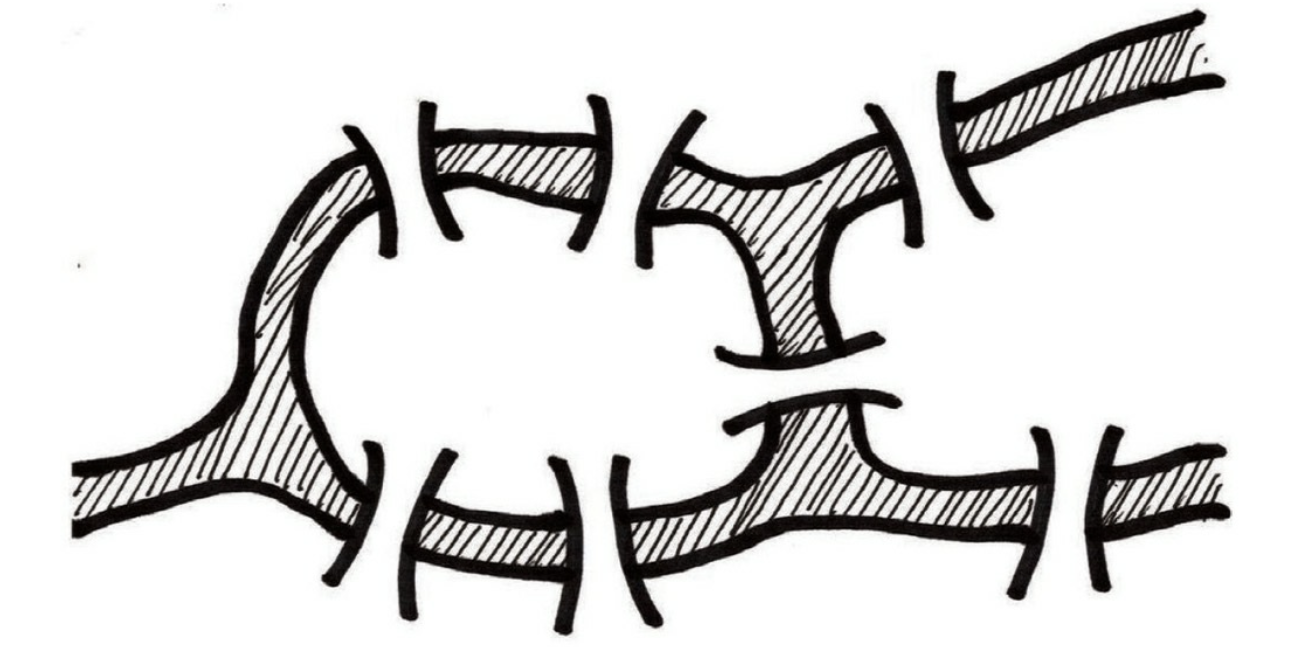
\includegraphics[width=.8\linewidth]{images/konigsberg.png}	
%\caption{Bridges of K\text{\"o}nigsberg.}
%\end{figure}
%\end{minipage} %
%\hfill 
%\begin{minipage}{.47\textwidth}
%\begin{figure}
%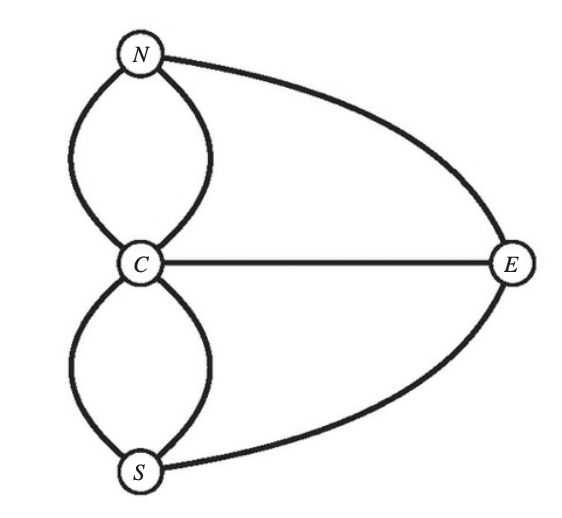
\includegraphics[width=.8\linewidth]{images/konigsberg_graph.png}
%\caption{Multi-graph representation}
%\end{figure}
%\end{minipage} %
%
%\vfill 
%\only<1>{\colorbox{blue!30}{\textbf{Terminology.}} A \textbf{Eulerian walk} is a walk that goes through every edge exactly once.}
%
%
%\only<2>{\colorbox{blue!30}{\textbf{Terminology.}} A \textbf{multigraph} is a graph in which multiple edges between the same pair of vertices are allowed. (Note: So a graph is a special case of a multi-graph.)}
%
%
%\end{frame}


\begin{frame}[t]{K\"onigsberg bridge problem}

\begin{columns}[T]
\begin{column}{0.47\textwidth}
\begin{minipage}[t][2.3cm]{\linewidth}
\raggedright
\colorbox{red!30}{\textbf{Question.}} Is there a tour of K\"onigsberg that traverses each bridge exactly once? 
\end{minipage}
\begin{figure}
\parbox[c][3.2cm][c]{\linewidth}{\centering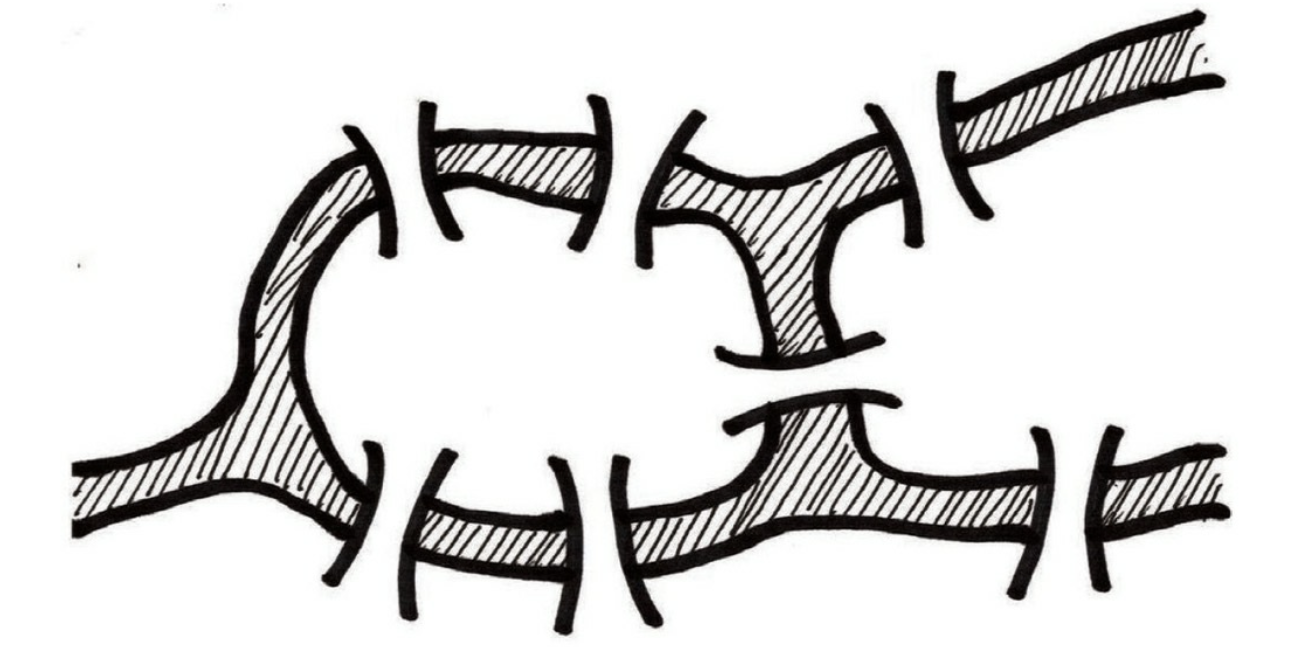
\includegraphics[width=.9\linewidth]{images/konigsberg.png}}
\caption{Bridges of K\"onigsberg.}
\end{figure}
\end{column}
\begin{column}{0.47\textwidth}
\begin{minipage}[t][2.3cm]{\linewidth}
\raggedright
\only<1>{\colorbox{blue!30}{\textbf{Graph Terminology.}} A \textbf{multigraph} is a graph in which multiple edges between the same pair of vertices are allowed.} %(Note: So a graph is a special case of a multi-graph.)
\only<2->{\colorbox{blue!30}{\textbf{Graph Terminology.}} A \textbf{Eulerian walk} is a walk that goes through every edge exactly once.}%
\end{minipage}
\begin{figure}
\parbox[c][3.2cm][c]{\linewidth}{\centering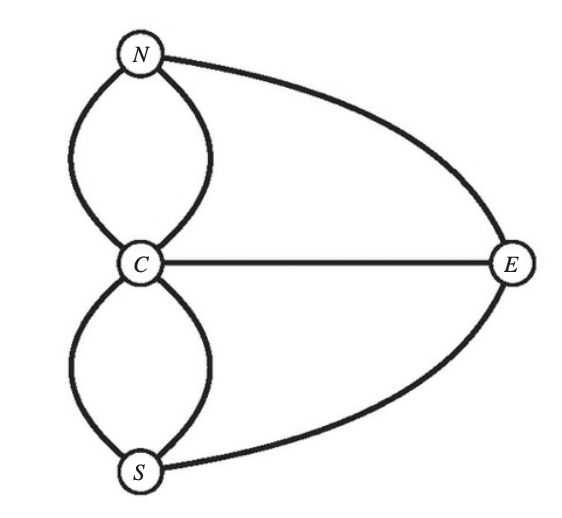
\includegraphics[height=3.2cm]{images/konigsberg_graph.png}}
\caption{Multi-graph representation}
\end{figure}
\end{column}
\end{columns}
\vspace{-.2cm}
\onslide<3->{%
\begin{mygreenbox}[title=Key point]
We want to know if this graph has a \textbf{Eulerian walk}.
\end{mygreenbox}}
\vspace{0.4cm}
\end{frame}


\begin{frame}{Solution to K\"onigsberg bridge problem}
 
 
\colorbox{yellow!30}{\textbf{Poll.}} Is there a tour of K\"onigsberg that traverses each bridge exactly once? 
\vfill 



 \begin{center}
 \scalebox{0.9}{
 \begin{tikzpicture}[
  vtx/.style={circle, draw, line width=0.8pt, fill=white, inner sep=1.5pt, minimum size=0.6cm},
  every edge/.style={draw, line width=1.2pt},
   bubble/.style={rectangle callout, rounded corners=3pt, draw=orange!80!black, fill=yellow!30, line width=0.6pt,
                 text width=2.1cm, align=center, font=\small, inner sep=3pt, callout pointer shorten=0.32cm, overlay}]]
  \node[vtx] (N) at (0, 2)   {$N$};
  \node[vtx] (C) at (0, 0)   {$C$};
  \node[vtx] (S) at (0,-2)   {$S$};
  \node[vtx] (E) at (3.6, 0) {$E$};
  % two bridges between N and C, and two between C and S
  \path (N) edge[bend right=45] (C)
        (N) edge[bend left=45]  (C)
        (C) edge[bend right=45] (S)
        (C) edge[bend left=45]  (S);
  % one bridge from each of N, C, S to E
  \path (N) edge[out=-10, in=105] (E)
        (C) edge                 (E)
        (S) edge[out=10, in=-105] (E);
        
  % degree labels, shown from the second overlay
  \node<2->[red, above=1pt]  at (N.north) {deg 3};
  \node<2->[red, left=4pt]   at (C.west)  {deg 5};
  \node<2->[red, below=1pt]  at (S.south) {deg 3};
  \node<2->[red, right=1pt]  at (E.east)  {deg 3};
  % callouts, one per reveal, placed outside the graph
  \node<3>[bubble, callout absolute pointer={(E)}] at (4.9, 1.3)    {If the walk starts elsewhere, it must end here.};
  \node<4>[bubble, callout absolute pointer={(E)}] at (4.9, 1.3)    {The walk must start or end here.};
  \node<5>[bubble, callout absolute pointer={(N)}] at (-2.0, 2.0)   {If the walk starts elsewhere, it must end here.};
  \node<6>[bubble, callout absolute pointer={(N)}] at (-2.0, 2.0)  {The walk must start or end here.};
  \node<7>[bubble, callout absolute pointer={(C)}] at (-2.2, 0.9)   {If the walk starts elsewhere, it must end here.};
   \node<8>[bubble, callout absolute pointer={(C)}] at (-2.2, 0.9)  {The walk must start or end here.};
  \node<9>[bubble, callout absolute pointer={(S)}] at (-2.0, -2.0)  {If the walk starts elsewhere, it must end here.};
   \node<10>[bubble, callout absolute pointer={(S)}] at (-2.0, -2.0)  {The walk must start or end here.};
\end{tikzpicture}
}
 \end{center}
 
\only<11>{%
\begin{myredbox}[title=Problem]
We cannot start or end the walk in each of the four districts!
\end{myredbox}}
 
  \only<12>{%
\begin{mybluebox}[title=Answer to Poll]
No, there is no tour of K\"onigsberg that traverses each bridge exactly once.
\end{mybluebox}}

 \only<13>{%
\begin{mygreenbox}[title=General Insight]
If a node $v$ has odd degree, every Eulerian walk must start or end at $v$.
\end{mygreenbox}}
 


 
\end{frame}




\begin{frame}{Eulerian walks}
 
 
 \begin{mygreenbox}[title=\text{Eulerian Walks (Theorem 7.3.1, Lovász)}]
If a connected graph...
\begin{itemize}
\item[a)] ...has more than two nodes with an odd degree, then it has no Eulerian walk.
\item[b)] ...has exactly two nodes with odd degree, then it has an Eulerian walk.  Every Eulerian walk must start at one of these and end at the other one.
\item[c)] ...has no nodes with odd degree, then it has an Eulerian walk.  Every Eulerian walk is closed.
\end{itemize}
\end{mygreenbox}

\vfill 

\only<1>{\colorbox{blue!30}{\textbf{Remarks.}} Case (a) is what we just reasoned through.  Case (b) is a group exercise.}

\only<2->{\colorbox{yellow!30}{\textbf{Poll.}} Why doesn't this theorem mention the case where a graph has exactly \textbf{one} node with odd degree?}

 \end{frame} 
 
 
 
\begin{frame}[t]{Eulerian Walk vs. Hamiltonian Path}
\footnotesize

\only<1>{\colorbox{yellow!30}{\textbf{Poll.}} What is the difference between a Eulerian Walk and a Hamiltonian Path?}

\only<2->{
% ---------- row 1: definitions ----------
\begin{columns}[T]
\begin{column}{0.48\textwidth}
\begin{mybluebox}[title=Eulerian walk]
\raggedright A walk that uses every \textbf{edge} exactly once.
\end{mybluebox}
\end{column}
\begin{column}{0.48\textwidth}
\begin{mybluebox}[title=Hamiltonian path]
\raggedright A path that visits every \textbf{vertex} exactly once.
\end{mybluebox}
\end{column}
\end{columns}

\vspace{0.15cm}
% ---------- row 2: example graphs ----------
\begin{columns}[T]
\begin{column}{0.48\textwidth}
\centering
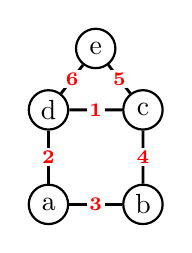
\begin{tikzpicture}[scale=0.6,
  vtx/.style={circle, draw, line width=0.8pt, fill=white, inner sep=1pt, minimum size=0.5cm},
  lbl/.style={red, font=\scriptsize\bfseries, fill=white, inner sep=1pt}]
  \node[vtx] (1) at (0,0)   {a};
  \node[vtx] (2) at (2,0)   {b};
  \node[vtx] (3) at (2,2)   {c};
  \node[vtx] (4) at (0,2)   {d};
  \node[vtx] (5) at (1,3.3) {e};
  % edges numbered in the order the walk 3, 4, 1, 2, 3, 5, 4 uses them
  \draw[line width=1pt] (3) -- node[lbl] {1} (4);
  \draw[line width=1pt] (4) -- node[lbl] {2} (1);
  \draw[line width=1pt] (1) -- node[lbl] {3} (2);
  \draw[line width=1pt] (2) -- node[lbl] {4} (3);
  \draw[line width=1pt] (3) -- node[lbl] {5} (5);
  \draw[line width=1pt] (5) -- node[lbl] {6} (4);
\end{tikzpicture}

Walk: $c, d, a, b, c, e, d$
\end{column}
\begin{column}{0.48\textwidth}
\centering
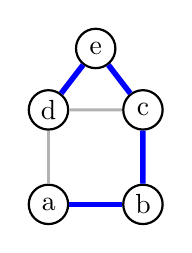
\begin{tikzpicture}[scale=0.6,
  vtx/.style={circle, draw, line width=0.8pt, fill=white, inner sep=1pt, minimum size=0.5cm},
  path/.style={blue, line width=2pt}]
  \node[vtx] (1) at (0,0)   {a};
  \node[vtx] (2) at (2,0)   {b};
  \node[vtx] (3) at (2,2)   {c};
  \node[vtx] (4) at (0,2)   {d};
  \node[vtx] (5) at (1,3.3) {e};
  % edges not on the path
  \draw[gray!60, line width=1pt] (3) -- (4);
  \draw[gray!60, line width=1pt] (4) -- (1);
  % the Hamiltonian path 1, 2, 3, 5, 4
  \draw[path] (1) -- (2);
  \draw[path] (2) -- (3);
  \draw[path] (3) -- (5);
  \draw[path] (5) -- (4);
\end{tikzpicture}

Path: $a, b, c, e, d$
\end{column}
\end{columns}
}

\vspace{0.05cm}

\begin{center}
\only<3>{\colorbox{red!30}{\large \textbf{Who cares?!}}}
\end{center}

\only<4>{
% ---------- row 3: complexity ----------
\begin{columns}[T]
\begin{column}{0.48\textwidth}
\begin{mygreenbox}[title=Complexity]
\raggedright \textbf{Easy.} Deciding whether one exists (and finding it) takes \textbf{linear time}, $O(|V| + |E|)$.
\end{mygreenbox}
\end{column}
\begin{column}{0.48\textwidth}
\begin{myredbox}[title=Complexity]
\raggedright \textbf{Hard.} Deciding whether one exists is \textbf{NP-complete}: no efficient algorithm is known.
\end{myredbox}
\end{column}
\end{columns}
}

\end{frame}


\begin{frame}[t]{Application: DNA Sequencing}
\footnotesize

\colorbox{blue!30}{\textbf{Problem.}} Sequencers can't read a whole genome at once.  They read millions of short, overlapping fragments (\textbf{reads}), which we must stitch back together.

\vspace{0.2cm}
\begin{columns}[T]
% ---------- Hamiltonian approach ----------
\begin{column}{0.48\textwidth}
\only<2->{
\textbf{Idea 1: Hamiltonian path}\\
Vertices = reads, edges = overlaps.  Find a path through every \textbf{vertex}.

\vspace{0.05cm}
\centering
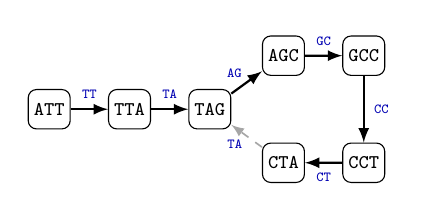
\begin{tikzpicture}[scale=0.85,
  v/.style={draw, rounded corners=3pt, font=\ttfamily\scriptsize, inner sep=2pt, minimum height=0.5cm},
  arr/.style={->, >=latex, line width=0.8pt},
  weak/.style={->, >=latex, line width=0.6pt, gray!70, dashed},
  el/.style={font=\ttfamily\tiny, text=blue!70!black}]
  \node[v] (ATT) at (-2.4, 0)  {ATT};
  \node[v] (TTA) at (-1.2, 0)  {TTA};
  \node[v] (TAG) at (0, 0)     {TAG};
  \node[v] (AGC) at (1.1, 0.8) {AGC};
  \node[v] (GCC) at (2.3, 0.8) {GCC};
  \node[v] (CCT) at (2.3,-0.8) {CCT};
  \node[v] (CTA) at (1.1,-0.8) {CTA};
  % the Hamiltonian path
  \draw[arr] (ATT) -- node[el, above] {TT} (TTA);
  \draw[arr] (TTA) -- node[el, above] {TA} (TAG);
  \draw[arr] (TAG) -- node[el, above left=-2pt] {AG} (AGC);
  \draw[arr] (AGC) -- node[el, above] {GC} (GCC);
  \draw[arr] (GCC) -- node[el, right] {CC} (CCT);
  \draw[arr] (CCT) -- node[el, below] {CT} (CTA);
  % an overlap the path doesn't use
  \draw[weak] (CTA) -- node[el, below left=-2pt] {TA} (TAG);
\end{tikzpicture}

{\scriptsize Visiting every vertex spells {\ttfamily ATTAGCCTA}.}
}

\vspace{0.2cm}
\raggedright
\only<3->{
\colorbox{red!30}{\textbf{NP-hard.}} Hopeless for millions of reads.
}
\end{column}
% ---------- Eulerian approach ----------
\begin{column}{0.48\textwidth}
\only<4->{
\textbf{Idea 2: Eulerian path} (de Bruijn graph)\\
Edges = reads, vertices = overlaps. Find a path through every \textbf{edge}.

%Chop reads into 3-letter pieces; each piece is an \textbf{edge}.  Find a path through every edge.
\vspace{0.05cm}
\centering
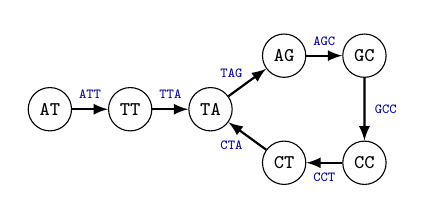
\begin{tikzpicture}[scale=0.85,
  v/.style={circle, draw, font=\ttfamily\scriptsize, inner sep=1pt, minimum size=0.55cm},
  arr/.style={->, >=latex, line width=0.8pt},
  el/.style={font=\ttfamily\tiny, text=blue!70!black}]
  \node[v] (AT) at (-2.4, 0)  {AT};
  \node[v] (TT) at (-1.2, 0)  {TT};
  \node[v] (TA) at (0, 0)     {TA};
  \node[v] (AG) at (1.1, 0.8) {AG};
  \node[v] (GC) at (2.3, 0.8) {GC};
  \node[v] (CC) at (2.3,-0.8) {CC};
  \node[v] (CT) at (1.1,-0.8) {CT};
  \draw[arr] (AT) -- node[el, above] {ATT} (TT);
  \draw[arr] (TT) -- node[el, above] {TTA} (TA);
  \draw[arr] (TA) -- node[el, above left=-2pt] {TAG} (AG);
  \draw[arr] (AG) -- node[el, above] {AGC} (GC);
  \draw[arr] (GC) -- node[el, right] {GCC} (CC);
  \draw[arr] (CC) -- node[el, below] {CCT} (CT);
  \draw[arr] (CT) -- node[el, below left=-2pt] {CTA} (TA);
\end{tikzpicture}

{\scriptsize Following every edge spells {\ttfamily ATTAGCCTA}.}
}
\only<5->{

\vspace{0.2cm}
\raggedright
\colorbox{green!30}{\textbf{Linear time.}} Used by modern genome assemblers.
}
\end{column}
\end{columns}

\vspace{0.12cm}
\only<6->{
\colorbox{blue!30}{\textbf{Key point.}} Same data, but switching from \qq{visit every \textbf{vertex}} to \qq{visit every \textbf{edge}} turns an intractable problem into an easy one.
}

\citebottom{Pevzner, Tang \& Waterman (2001). An Eulerian path approach to DNA fragment assembly. \textit{PNAS}, 98(17), 9748--9753.}
\end{frame}


\begin{frame}[standout]
Group Exercises
\end{frame}

\begin{frame}{Random Group Assignments}
%%% TABLE 1: by last name
\begin{columns}
\begin{column}{0.33\textwidth}
Ashley, Isabelle: 9 \\ 
Bailey, Tanna: 8 \\ 
Blaisdell, Olyver: 4 \\ 
Brown, Ashton: 9 \\ 
Cardenas, Dominic: 5 \\ 
Cutler, George: 8 \\ 
Fabik, Roland: 6 \\ 
Fuller, Ryan: 7 \\ 
Griffen, Clara: 1 \\ 
Grutsch, Tanner: 8 \\ 
Hager, Nathan: 4 \\\end{column}
\begin{column}{0.33\textwidth}
Horner, Jayden: 5 \\ 
Johnson, Jaret: 2 \\ 
Kintzel, Samantha: 1 \\ 
Lameres, Alexis: 2 \\ 
Lee, Holden: 11 \\ 
Mayala, Reece: 10 \\ 
McLean, Connor: 7 \\ 
Mcbride, Daniel: 6 \\ 
Miller, Maverick: 1 \\ 
Moss, Emily: 11 \\ 
Mousseau, Matthew: 7 \\\end{column}
\begin{column}{0.33\textwidth}
Neuman, Evan: 10 \\ 
Putnam, John: 10 \\ 
Rathbun, Jedidiah: 3 \\ 
Roberts, Matthew: 3 \\ 
Roller, Nathan: 3 \\ 
Ryan, Otis: 9 \\ 
Shevtsov, Timothy: 11 \\ 
Stensland, Emma: 6 \\ 
Thiessen, Logan: 4 \\ 
Thompson, Jaiden: 2 \\ 
Vath, Ethan: 5 \\\end{column}
\end{columns}	
\end{frame}

\begin{frame}{Group Exercises}

\begin{enumerate}
	\item Which of these graphs has an Eulerian walk? Which have a closed Eulerian walk?  Find a Eulerian walk if it exists.
	\begin{center}
	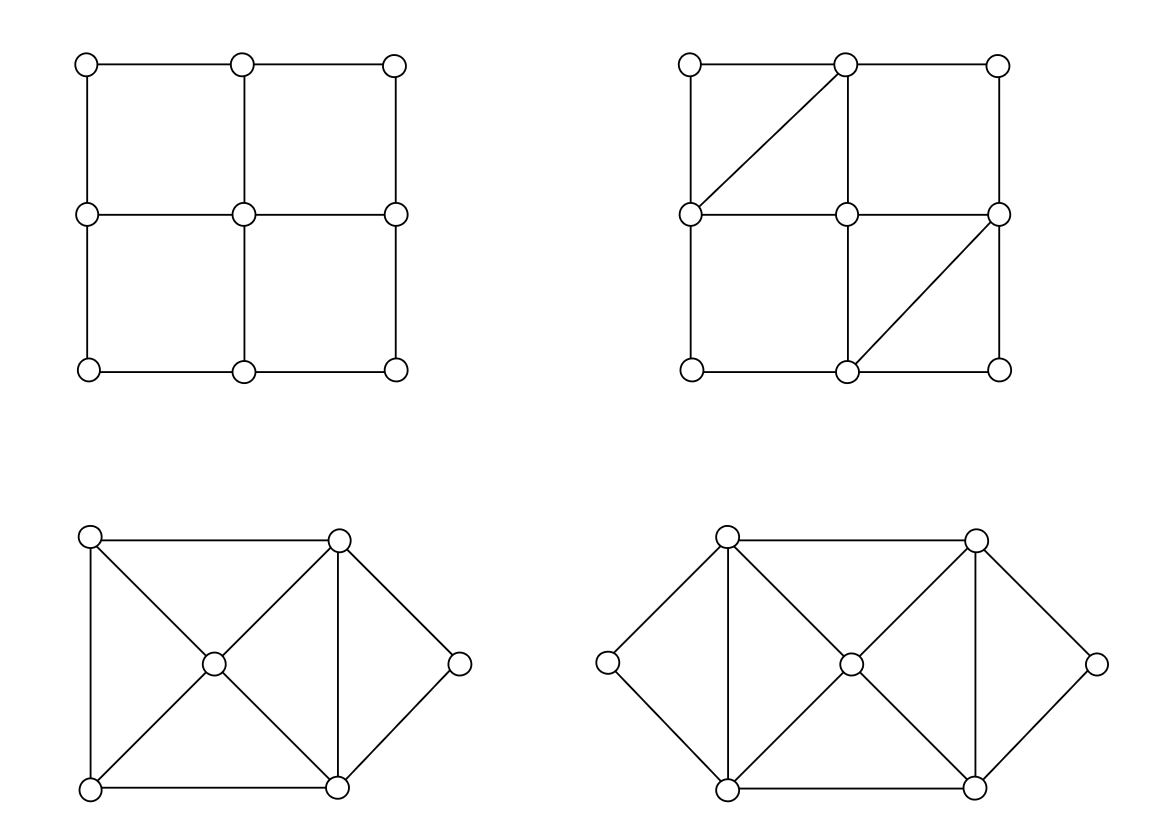
\includegraphics[height=0.4\textheight]{images/eulerian_walk_puzzle.png}
	\end{center}
	\item Prove the first statement of part (b) of the theorem below.  You may assume parts (a) and (c), which were proved in the text.
\end{enumerate}


\tiny 
 \begin{mygreenbox}[title=\text{Eulerian Walks (Theorem 7.3.1, Lovász)}]
If a connected graph...
\begin{itemize}
\item[a)] ...has more than two nodes with an odd degree, then it has no Eulerian walk.
\item[b)] ...has exactly two nodes with odd degree, then it has an Eulerian walk.  Every Eulerian walk must start at one of these and end at the other one.
\item[c)] ...has no nodes with odd degree, then it has an Eulerian walk.  Every Eulerian walk is closed.
\end{itemize}
\end{mygreenbox}

\end{frame}


\begin{frame}{Solution to Group Exercise \#1}
\small 
\textbf{Problem.} Which of these graphs has an Eulerian walk? Which have a closed Eulerian walk?  Find a Eulerian walk if it exists.
	\begin{center}
	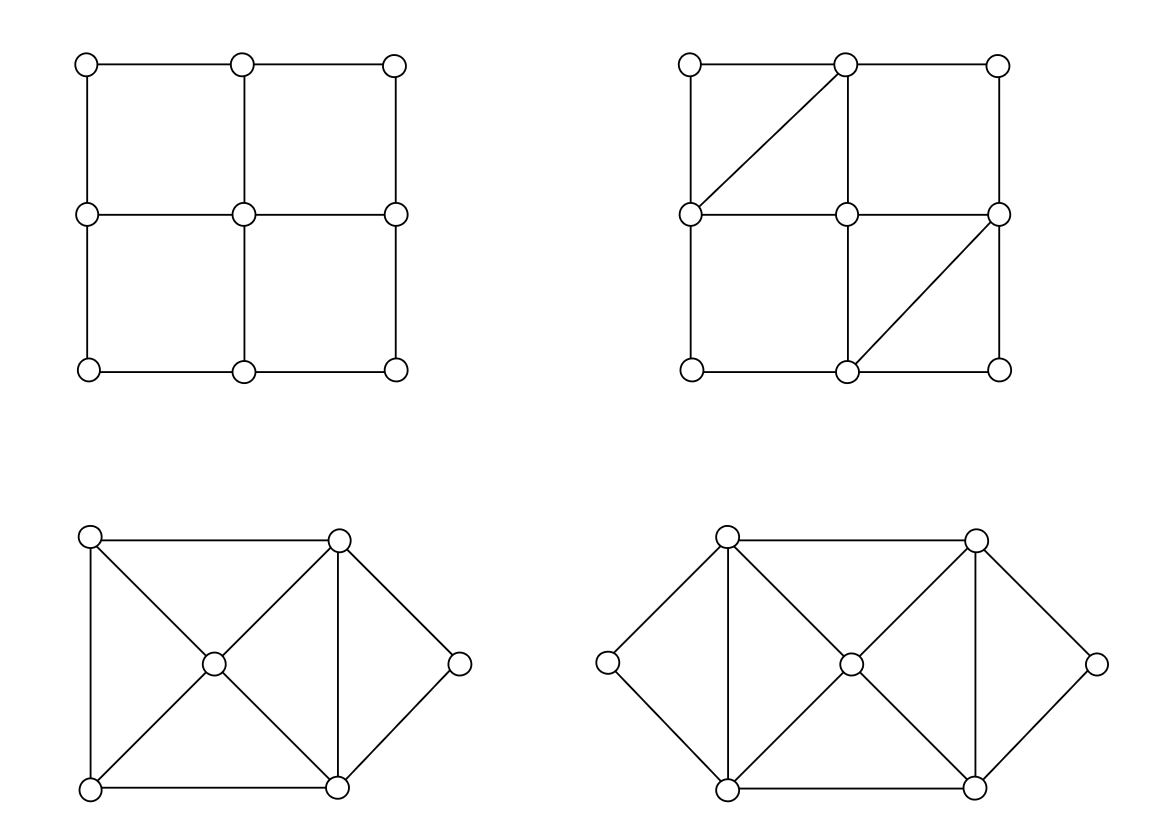
\includegraphics[height=0.4\textheight]{images/eulerian_walk_puzzle.png}
	\end{center}
\textbf{Solution.}  We can solve this problem by applying the theorem. Top Left: No. Bottom Left: Yes. Top Right: Yes, and it's closed. Bottom Right: Yes, and it's closed.
\tiny 
 \begin{mygreenbox}[title=\text{Eulerian Walks (Theorem 7.3.1, Lovász)}]
If a connected graph...
\begin{itemize}
\item[a)] ...has more than two nodes with an odd degree, then it has no Eulerian walk.
\item[b)] ...has exactly two nodes with odd degree, then it has an Eulerian walk.  Every Eulerian walk must start at one of these and end at the other one.
\item[c)] ...has no nodes with odd degree, then it has an Eulerian walk.  Every Eulerian walk is closed.
\end{itemize}
\end{mygreenbox}

\end{frame}

\begin{frame}{Solution to Group Exercise \#2}

\scriptsize  
\textbf{Problem.} Prove the first statement of part (b) of the theorem below.  You may assume parts (a) and (c), which were proved in the text.


\tiny 
 \begin{mygreenbox}[title=\text{Eulerian Walks (Theorem 7.3.1, Lovász)}]
If a connected graph...
\begin{itemize}
\item[a)] ...has more than two nodes with an odd degree, then it has no Eulerian walk.
\item[b)] ...has exactly two nodes with odd degree, then it has an Eulerian walk.  Every Eulerian walk must start at one of these and end at the other one.
\item[c)] ...has no nodes with odd degree, then it has an Eulerian walk.  Every Eulerian walk is closed.
\end{itemize}
\end{mygreenbox}

\scriptsize  

\textbf{Solution.}  

\begin{enumerate}
	\item  Make a new multigraph $G'$ by adding one new edge $e$ between $u$ and $v$.
\item In $G'$, every vertex of $G'$ has even degree.
\item $G'$ is connected, because $G$ is and we only added an edge.
\item By the closed-walk result, $G'$ has a closed Eulerian walk $C$. Because $C$ is closed, we can start reading it at any of its vertices. Read it so that its last edge is $e$:
\[ C = u,\ \dots,\ v,\ e,\ u.\]
\item Delete that final edge $e$. What remains is a walk from $u$ to $v$ that uses every edge of $G$ exactly once. That is an Eulerian walk in $G$.
\end{enumerate}	




	
\end{frame}


\end{document}
